% The residue-field column added to the prime-above picture: the
% quotients 𝒪_K/𝔭 ≅ 𝔽_{p^f} over 𝔽_p are finite fields.
% Source: book/tex/alg-NT/ramification.tex (§ (Optional)
% Decomposition and inertia groups) — tikzcd.
\documentclass[border=2mm]{standalone}
\usepackage{tikz}
\usepackage{amssymb}
\begin{document}
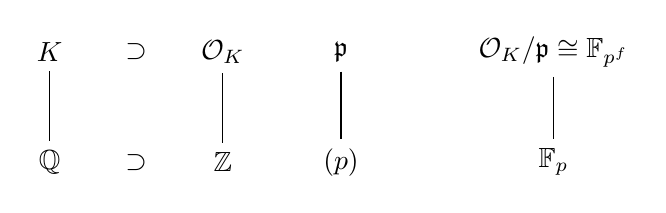
\begin{tikzpicture}
  \node (K) at (0,1.4) {$K$};
  \node (Q) at (0,0) {$\mathbb{Q}$};
  \node (s1) at (1.1,1.4) {$\supset$};
  \node (s2) at (1.1,0) {$\supset$};
  \node (OK) at (2.2,1.4) {$\mathcal{O}_K$};
  \node (Z) at (2.2,0) {$\mathbb{Z}$};
  \node (pi) at (3.7,1.4) {$\mathfrak{p}$};
  \node (p) at (3.7,0) {$(p)$};
  \node (q1) at (6.4,1.4) {$\mathcal{O}_K/\mathfrak{p} \cong \mathbb{F}_{p^f}$};
  \node (q2) at (6.4,0) {$\mathbb{F}_p$};
  \draw (K) -- (Q);
  \draw (OK) -- (Z);
  \draw (pi) -- (p);
  \draw (q1) -- (q2);
\end{tikzpicture}
\end{document}
